\documentclass[a4paper,utf8]{article}
\usepackage{graphicx}
\usepackage[heading,fancyhdr]{ctex}
\usepackage{amsmath,amssymb,geometry,ulem}
\usepackage{array,tabularx,tabulary,mhchem,xspace}
\usepackage{floatrow,subfig,multirow,bigstrut}
\usepackage{siunitx,booktabs,longtable,nameref}
\lineskiplimit=1pt
\lineskip=3pt
\geometry{
    top=25.4mm, 
    left=25mm, 
    right=25mm, 
    bottom=25mm,
    headsep=5.9mm,
}
\ctexset{
    chapter = {
        name = {实验,},
        beforeskip = {-23pt}
    }
}
\newcommand{\fgref}[1]{图~\ref{#1}\xspace}
\newcommand{\seqref}[1]{式~(\ref{#1})}
\newcommand{\expinfo}[6][无]{
    {\zihao{-3}\bfseries\songti
    实验名称:\uline{\hfill\mbox{#2}\hfill} \\[2.9mm]
    学\quad 号:\uline{\makebox[25mm]{#3}}\hfill
    姓\quad 名:\uline{\makebox[25mm]{#4}}\hfill
    班\quad 级:\uline{\makebox[25mm]{#5}} \\[2.9mm]
    合作者:\uline{\makebox[25mm]{#1}} \hfill
    桌\quad 号:\uline{\makebox[25mm]{}}\hfill\makebox[25mm+4em]{}\\[2.9mm]
    指导教师:\uline{\makebox[30mm]{#6}}\hfill\mbox{} \\[2.9mm]
    实验日期:\uline{\makebox[30mm]{}}\hfill\mbox{} \\[58.7mm]
    }
}%\expinfo[合作者]{实验名称}{学号}{姓名}{班级}{指导教师}
\newcommand{\pointingbox}{
    {\zihao{4}\bfseries\songti%
    实验考核\\[3mm]
    \extrarowheight=3mm
    \begin{tabularx}{150mm}{|X|X|X|X|X|}\hline
        \hfil 项目 \hfil  & \hfil 实验预习 \hfil & \hfil 实验过程 \hfil & \hfil 分析与讨论 \hfil & \hfil 总评 \hfil \\[3mm] \hline
        \hfil 评价 \hfil &  &  &  &  \\[3mm] \hline
    \end{tabularx}
    }
}
\newcommand{\derivative}[2]{\frac{\mathrm{d} #1}{\mathrm{d} #2}}
\newcommand{\thinking}[2]{\textbf{#1}\\
答:\begin{minipage}[t]{0.85\textwidth}
    #2
\end{minipage}}

\pagestyle{fancy}
\fancyhf{}
%\fancyhead[C]{材料科学基础实验}
%\fancyfoot[C]{\thepage}
\fancyhead[EC]{\leftmark} \fancyhead[OC]{\rightmark}
\fancyhead[EL,OR]{\thepage}
\fancypagestyle{plain}{\renewcommand{\headrulewidth}{0pt}\fancyhf{}}

\newcounter{Rownumber}
\newcommand*{\Rown}{\stepcounter{Rownumber}\theRownumber}
\newcounter{sample}
\newcommand*{\Sam}{\stepcounter{sample}\thesample}
\newcounter{Fignumber}
\newcommand*{\Fign}{\stepcounter{Fignumber}\theFignumber}

\newcommand*{\resetRown}{\setcounter{Rownumber}{0}}
\newcommand{\qrange}[3]{\qtyrange[range-phrase = \text{$\sim$},range-units =single]{#1}{#2}{#3}}
\floatsetup[table]{capposition=top}
\newcolumntype{C}{>{\hfil}X<{\hfil}}
\renewcommand{\Nameref}[1]{\textbf{\ref{#1}~\nameref{#1}}}
\newcommand{\TTR}[0]{\watt\per\m\per\K} %导入导言
\begin{document}
\begin{center}
    {\mbox{}\\[7em]\zihao{2}\bfseries\songti%
    材料科学基础实验预习报告}\\[34mm]
    \expinfo{金属材料机械性能测量:拉伸和压缩
    }{22301077}{张蕴东}{22高分子}{李继玲}
\end{center}
\newpage
\part{拉伸实验}
\section{实验目的}
\begin{itemize}
    \item 了解电子万能试验机的基本结构、工作原理及使用方法;
    \item 观察拉伸时所表现的各种现象;
    \item 观察低碳钢和铸铁的断口特征,辨别两种材料的力学特征;
    \item 通过低碳钢和铸铁的应力-应变曲线,评价二者的力学性能,掌握金属材料屈服强度,抗拉强度,断裂伸长率和断面收缩率的测定方法。
\end{itemize}
\section{实验原理}%简单描述,含必要的公式和附图;
\subsection{低碳钢拉伸的应力-应变曲线及特征参数}
\subsubsection{低碳钢拉伸的应力-应变曲线}
低碳钢是塑性材料的典型代表性材料,对于低碳钢试样,在受拉伸过程中,如\fgref{fig:1} 所示应力-应变曲线,可以观察到试样经历四个典型的变形阶段:弹性变形阶段,屈服阶段,均匀塑性变形阶段(强化阶段),局部塑性变形阶段(颈缩阶段),伴随着应力-应变曲线上存在不同的特征点。
\begin{figure}[!ht]
    \begin{floatrow}\centering
        \ffigbox{\caption{低碳钢的拉伸曲线(R-e 曲线)\label{fig:1}}}{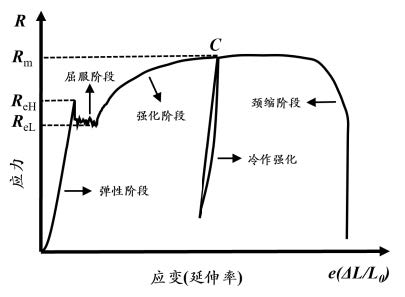
\includegraphics[height=50mm]{1.jpg}}
        \ffigbox{\caption{铸铁的拉伸曲线\label{fig:2}}}{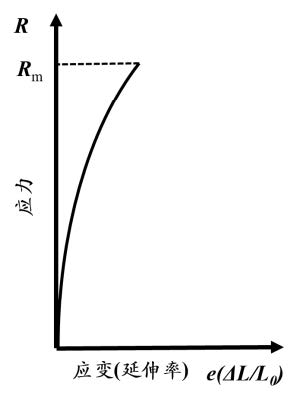
\includegraphics[height=50mm]{2.jpg}}
    \end{floatrow}
\end{figure}
\subsubsection{铸铁的应力-应变曲线}
铸铁是典型的脆性材料,铸铁的拉伸变形无屈服现象和缩颈现象,进行非常小的塑性变形后在较小的应力作用下就可被拉断,且突然断裂。拉断后铸铁的延伸率通常很小,约为 0.5\%。\fgref{fig:2} 为铸铁典型的应力-应变曲线,由图可见,铸铁的应力-应变曲线没有明显的直线部分。铸铁拉断前承受的最大应力值为其被拉伸的强度极限,定义为铸铁的抗拉强度。
\subsection{相关概念基本定义及计算公式}
\noindent 弹性模量:在应力-应变曲线上,应力低于弹性极限的范围内,应力与应变的比值,表达式为:\linebreak $E =\displaystyle \frac{\sigma}{\varepsilon}$,$\sigma$ 为应力,$\varepsilon$ 为应变。\\
上屈服强度 $R_{eH}$:试样发生屈服时应力下降时达到的最大值。\\
下屈服强度 $R_{eL}$:试样屈服期间屈服平台上不计初始屈服瞬时效应的最低应力点。\\
抗拉强度 $R_m$:试样缩颈前所达到的最大应力值。\\
原始标距 $L_0$:试样初始状态,夹头内用于测试的等截面积的试样部分的长度。\\
断后标距 $L_u$:实验被拉断后,将试样断口处紧密对接,初始标线内的总长度。\\
断后延伸率 $\delta$:试样拉断后,试样原始标线之间的伸长量和原始标距之比,$\delta = \displaystyle\frac{L_u-L_0}{L_0}\times 100\%$。\\
断面收缩率 $\psi$:试样拉断后,断口处横截面积的最大缩小量与原始标距内截面积之比,\linebreak $\psi = \displaystyle\frac{L_0-L_u}{L_0}\times 100\%$。
\section{实验仪器}%规格及参数
电子万能试验机,控制微机,游标卡尺,YYU-25/50 电子引伸计,低碳钢标准试样,铸铁标准试样。
\section{实验过程}%简述主要过程和实验内容
\begin{enumerate}
    \item .首先,在装夹试样前,标记待测试样的原始标距 $L_0$。选取待测试样夹头内部变形部分偏中间位置,在此处不同位置处选择3~5个截面,用游标卡尺在每个截面相互垂直的两个方向上分别测量一次该截面的直径,对所测量的所有截面直径求平均值即可视为待测试样拉伸之前的直径,记为 $d_0$,之后在待测试样夹头中间变形部分,以其变形部分的中点为中心,左右各选取 $5d_0$ 共 $10d_0$ 的长度,在端点处做标记,标记内即为待测试样的原始标距 $L_0$。
    \item 检查并确认电子万能试验机和计算机已连接。之后打开万能电子试验机,旋转红色急停旋钮使其弹起。
    \item 安装拉伸模具。
    \item 装夹试样。
    \item 装夹引伸计(低碳钢拉伸)。
    \item 编辑实验方案进行并进行测量。
    \item 进行测试
    \item 测量断后试样尺寸
    \item 保存数据,作图并分析待测试样各力学性能参数指标。
    \item 测量铸铁的拉伸曲线。
    \item 根据测量的低碳钢和铸铁的拉伸曲线,分析和判断两类金属材料的力学性能和各性能指标参数。
\end{enumerate}
\section{实验数据}
\part{压缩实验}
\end{document}
